\section{Result}
\label{result}

To compare the results shown in the article \cite{liu2010}, we test our implementation for all reported cases in the article. All the tests reported below are executed on Pianosa\footnote{Pianosa web site: \url{http://pianosa.di.unipi.it/Home_pianosa/html/info.html}}, the Computer Science Department's Cluster in Pisa. The cluster is composed by 24 homogeneous nodes. The nodes are 800 Mz Pentium III with 1GB of main memory and they are connected together through a Fast Ethernet interconnection network. On that cluster, we installed an Apache Hadoop 0.20.2 framework. The configuration parameters are set to default, so, the maximum number of task per node is set to 2 and the number of replication is set to 3. In our configuration, we decide to place the secondary node and the job tracker in cluster interface node that is not used also as task tracker. Only other 21 nodes are available as slave, cause to momentarily unavailability of the other nodes.

The data used in the test are generated by two matrix generators written in Matlab: one for the matrix A and other one for the matrices W and H. Both generators produce positive elements Gaussian distributed. The first one is a sparse matrix generator and its sparsity factor can be tuned through an input parameter. The second one, instead, is a complete matrix generator. For our tests, we fix the $m$ and $n$ parameters (the dimension of the A matrix) respectively to $105000$ and $20000$.

For all the test we did, the reduce task number is set to $ 1,8 * number\_of\_worker$, except in the phase 3 and 4 that have a fixed number of reduce tasks. This choice has been driven by the Hadoop User Guide that suggest to set the reduce task number to $$ mapred.map\_reduceMaximumTask * number\_of\_worker * C $$ where C is a constant choose in the range $[ 0.9, 1.8]$. For a value chosen in that range, it claim that the number of reduce tasks is optimal. In our experiments, we set that constant C to 0.9. Also for the first  W/H update, the input file number can be set in the proper way. In fact, the External Phase classes (that convert the input data from text to sequence) allow to specify how many reducer tasks must be used. In that way, an equal number of file are produced.

The first test battery done tests how the computation scales in relation to the the size of the data submitted. So, we study how the performances change varying the sparsity factor of the A matrix and setting different k values. In the first test, the number of non-zero elements in the sparse matrix has been changed between $5000000$ and $80000000$ elements while the k parameter remain fixed to 10. In the second one, instead, the k value has been varied between 10 and 125 while the non zero element of the A matrix has been fixed to $16500000$.  Both tests have been executed with 16 slave nodes for three iterative updates. The mean completion time of one iterative W/H update is reported in the figure \ref{DeltaVar}  and \ref{kVar}. 


\begin{figure}[th]
	\centerline{
		\mbox{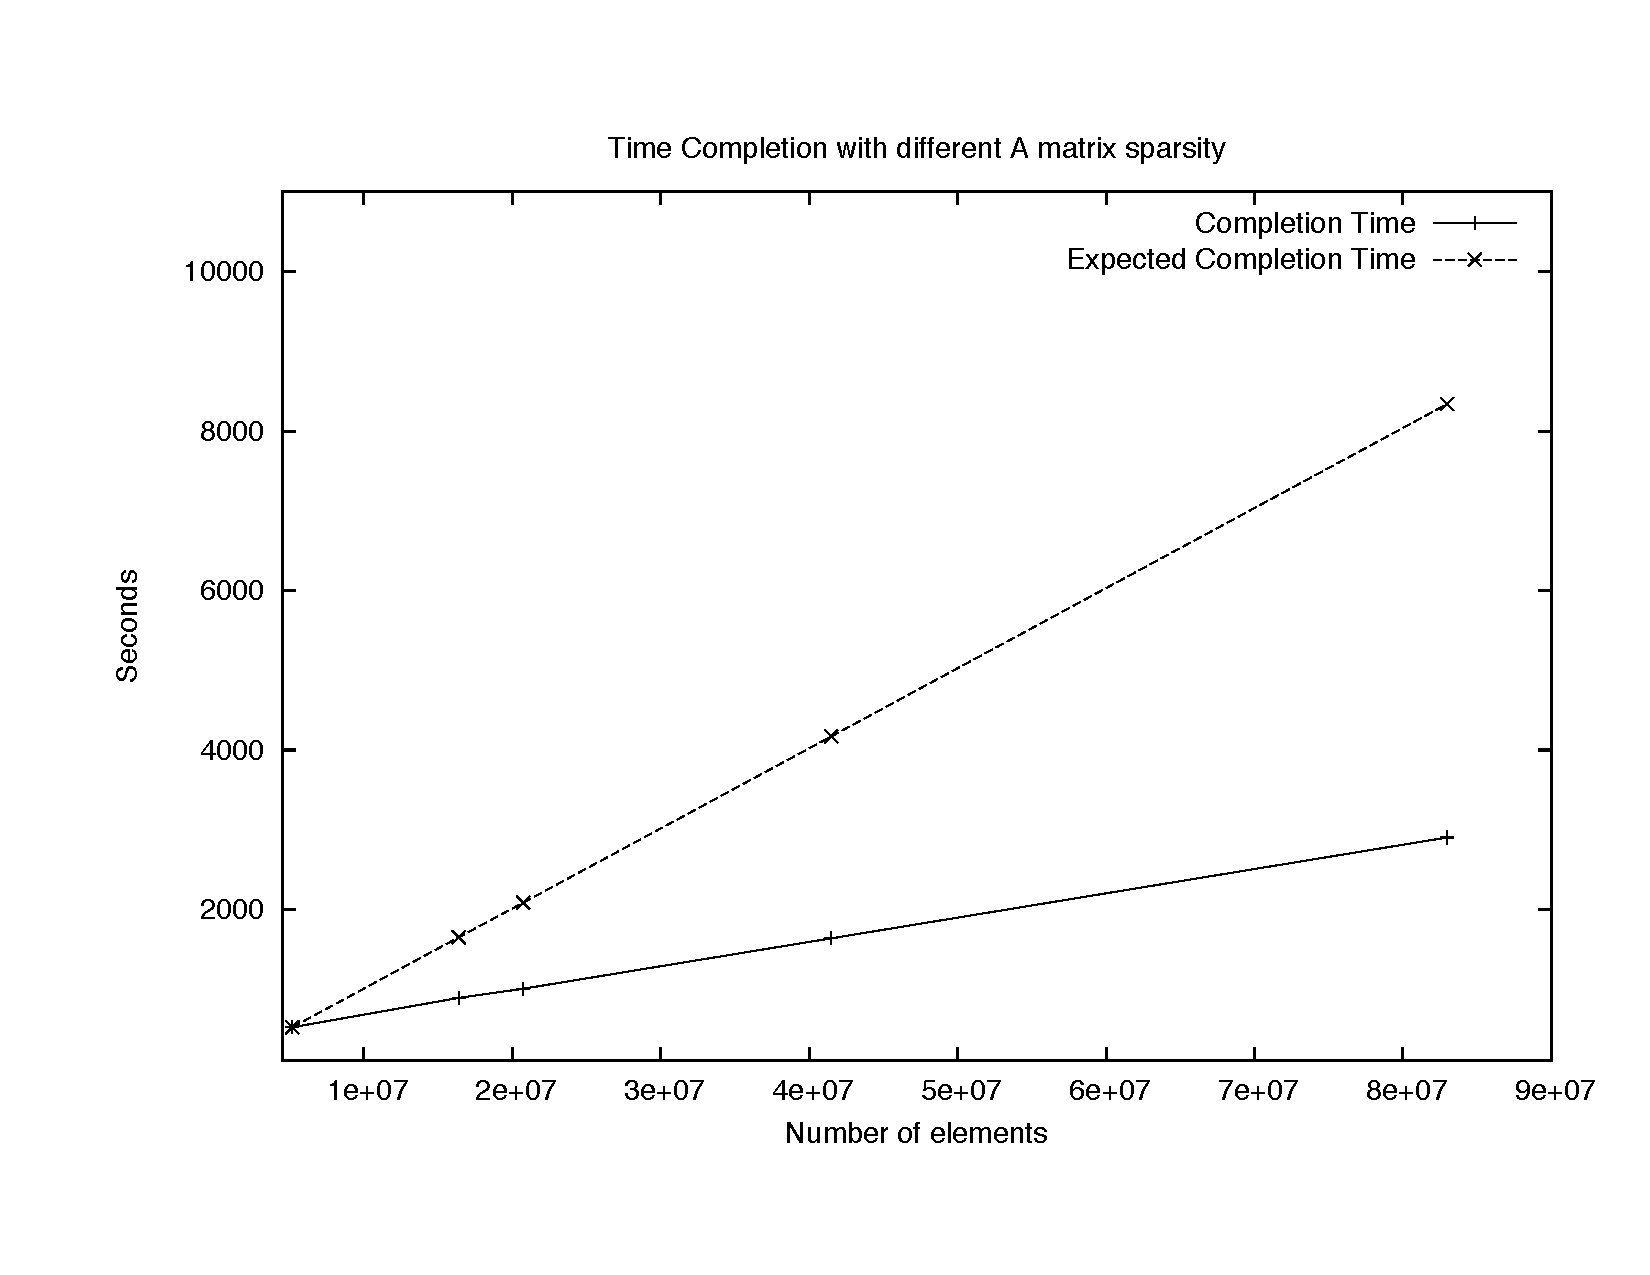
\includegraphics[scale=0.48]{HadoopTest/PsFiles/DeltaVar.pdf}}
	}
	\caption{Time Completion with different A matrix sparsity} 
        \label{DeltaVar}
\end{figure}

\begin{figure}[th]
	\centerline{
		\mbox{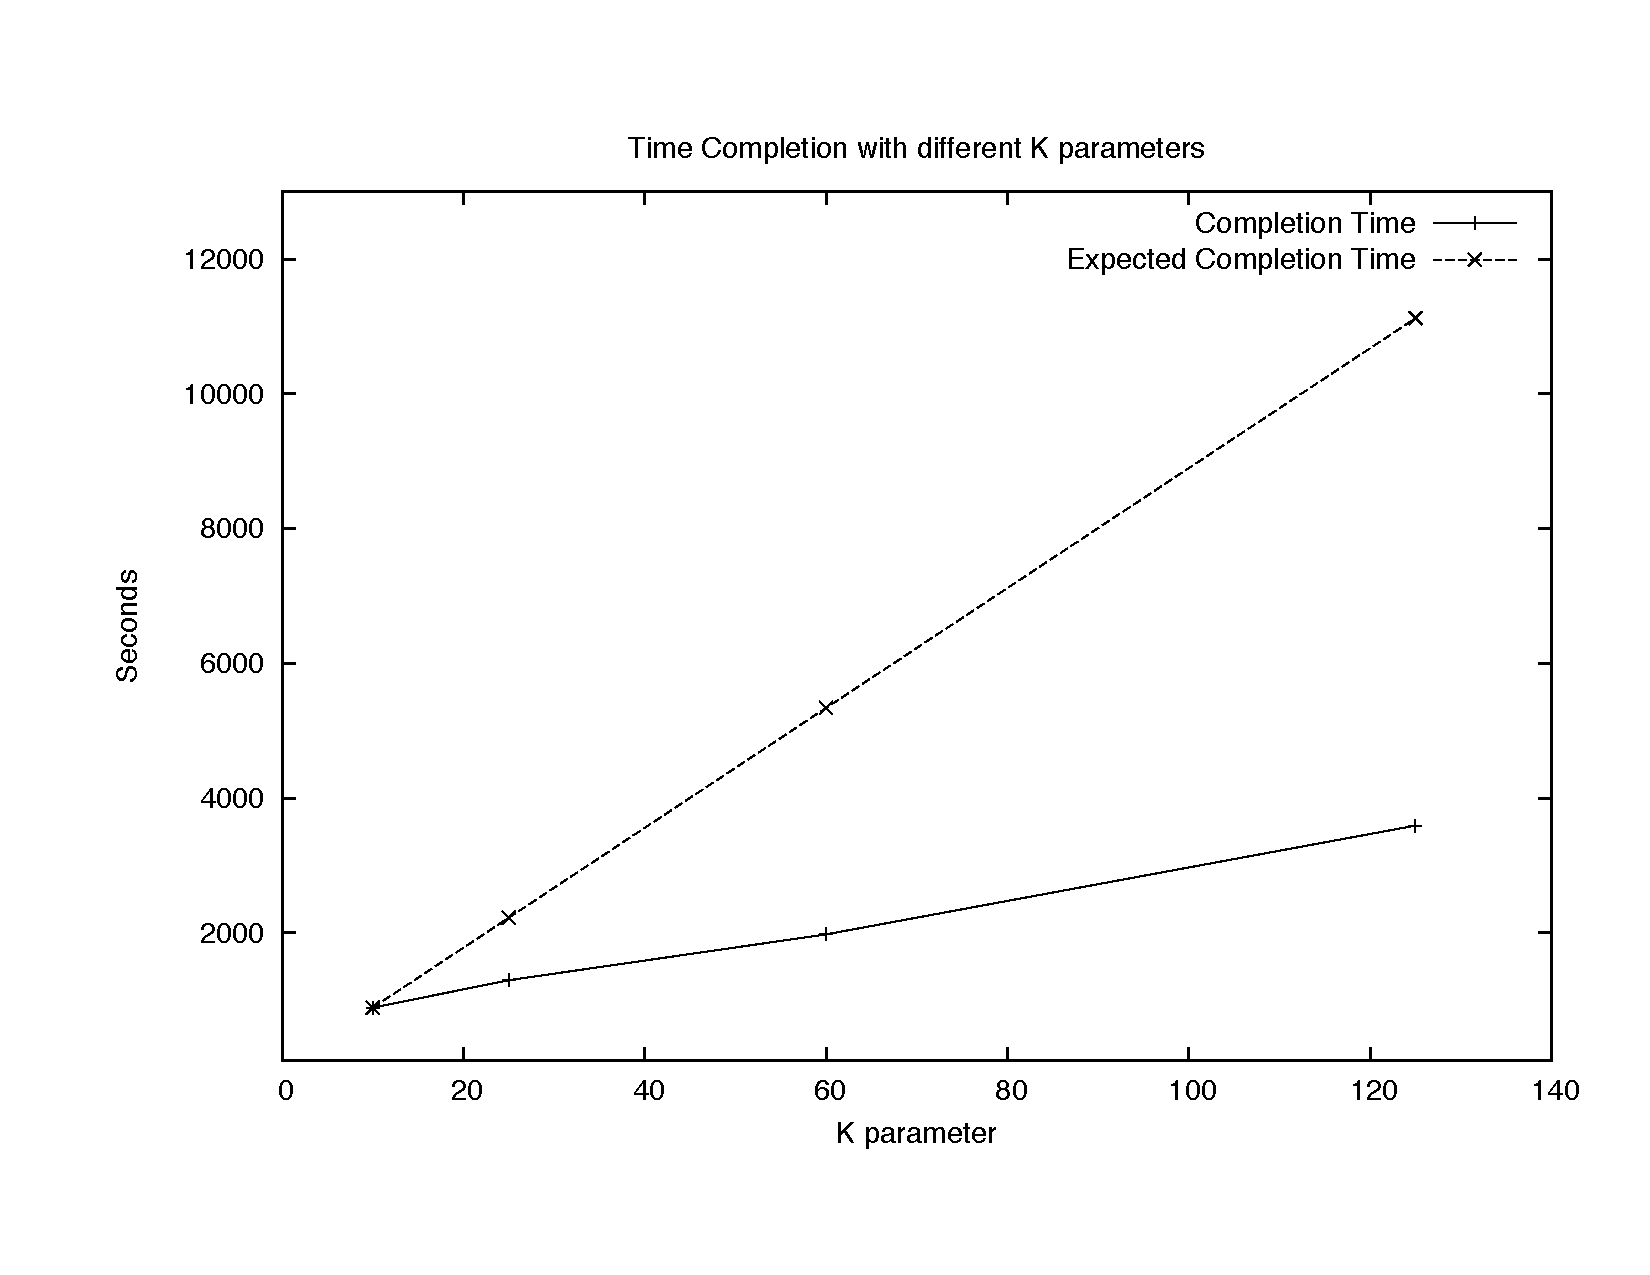
\includegraphics[scale=0.48]{HadoopTest/PsFiles/kVar.pdf}}
	}
	\caption{Time Completion with different K parameters} 
        \label{kVar}
\end{figure}


As we can see from both graphs, the behaviour of the test show a sub-linear dependencies from the size of the input data. \\

The second test battery points to examine the behaviour of the implementation when the parallel degree of the computation vary in the range $[1, 21]$. The results of the test are reported in the figure \ref{NTime}  and \ref{NScal}. The first graph focuses the attention on the completion time while the second one on the scalability.


\begin{figure}[th]
	\centerline{
		\mbox{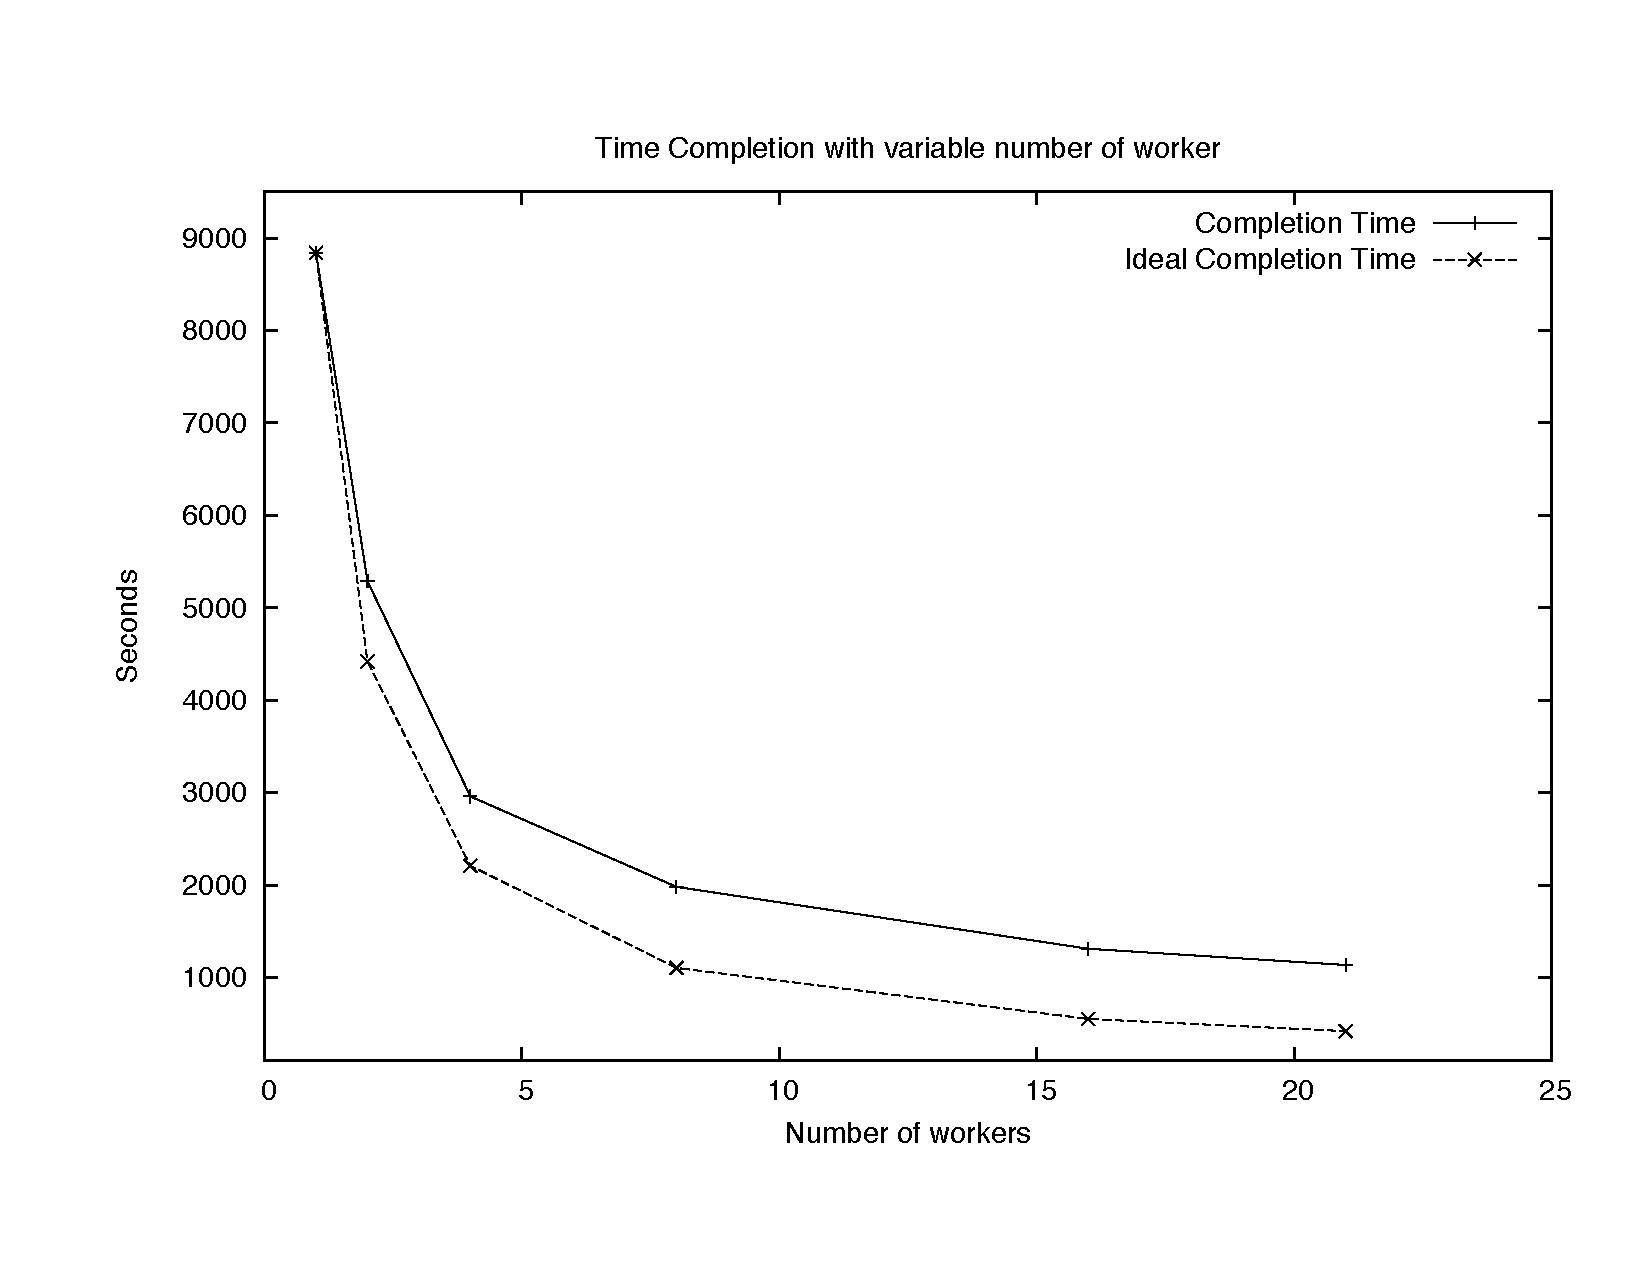
\includegraphics[scale=0.48]{HadoopTest/PsFiles/NTime.pdf}}
	}
	\caption{Time Completion with variable number of worker} 
        \label{NTime}
\end{figure}

\begin{figure}[th]
	\centerline{
		\mbox{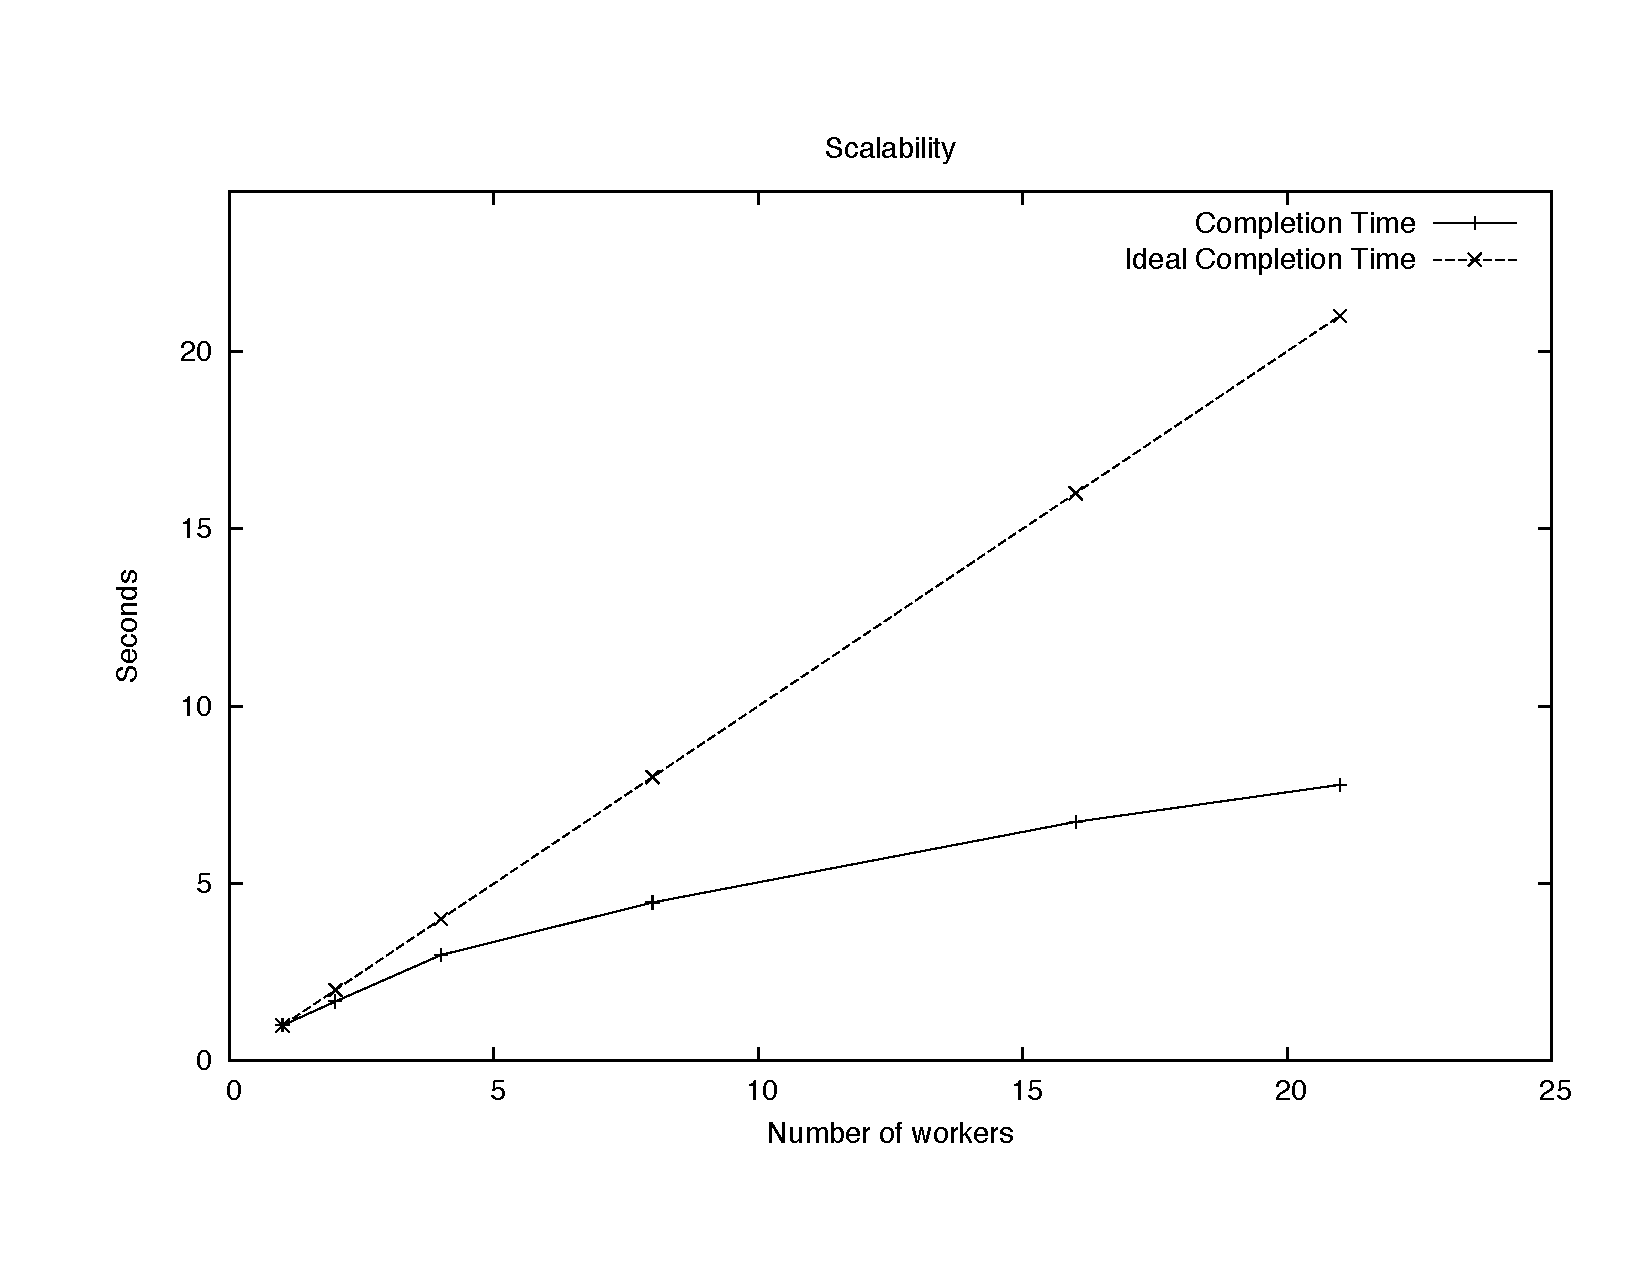
\includegraphics[scale=0.48]{HadoopTest/PsFiles/NScal.pdf}}
	}
	\caption{Scalability} 
        \label{NScal}
\end{figure}

As we can see from the figure \ref{NScal}, the implemented algorithm doesn't scale vary well. This is due mainly to two different facts: some phases in the computation doesn't scale adding more slave nodes and other phases, instead, doesn't exhibit an optimal scalability. An example of a phase that doesn't scale is the phase 5 (in which point-wise multiplication/division are done) has a minimal computational grain, both for map and reduce, and the most time spent in the computation reside in the shuffle phase. In a test we did with a parallel degree equals to 16, a shuffle task lasts in average 29 seconds, while a map and the reduce task end respectively in 8 and 3 seconds. This scenario is further compromise, taking in account that the completion time is given by the sequentialization of 5 different parallel phases. %The below table show the percentage that every phase in the computation takes varying the parallel degree.
The table reported below shows the average completion time for each phase varying the parallel degree.

\begin{center}
\begin{tabular}{ | l || c | c | c | c |  c | c | }
  \hline      
  Phase & 1 & 2 & 4 & 8 &16 & 21 \\
  \hline      
  Phase 1 & 2242 & 1492 & 797 & 469 & 320 & 304\\
  Phase 2 & 1678 & 885 & 478 & 303 & 191 & 148\\
  Phase 3 & 92 & 66 & 48 & 49 & 33 & 30\\ 
  Phase 4 & 23 & 19 & 21 & 27 & 20 & 20\\
  Phase 5 & 66 & 50 & 55 & 91 & 54 & 55\\
  \hline  
\end{tabular} 
\end{center}




%\begin{center}
%\begin{tabular}{ | l || c | c | c | c |  c | c | }
%  \hline      
%  Phase & 1 & 2 & 4 & 8 &16 & 21 \\
%  \hline      
%  Phase 1 & 0,512 & 0,557 & 0,542 & 0,476 & 0,494 & 0,510\\
%  Phase 2 & 0,446 & 0,390 & 0,374 & 0,356 & 0,341 & 0,300\\
%  Phase 3 & 0,015 & 0,019 & 0,026 & 0,043 & 0,047 & 0,051\\ 
%  Phase 4 & 0,006 & 0,009 & 0,015 & 0,028 & 0,030 & 0,036\\
%  Phase 5 & 0,016 & 0,023 & 0,041 & 0,095 & 0,086 & 0,101\\
%  \hline  
%\end{tabular}
%\end{center}

Furthermore, we make additional test to verify that the assumption done during the project were verified. The first one regards the coding of the data in sequential file during the ``internal phases''. The data shown in the below table show the completion time in the case the data are represented in the sequential or textual way. We can observe that coding the data provide a lot of benefits in the completion time, especially for the phase 1 and 2.

\begin{center}
\begin{tabular}{ | l || c | c | }
  \hline      
  & Text & Sequence \\
  \hline      
  Phase 1 & 475 & 264 \\
  Phase 2 & 333 & 105 \\
  Phase 3 & 66 & 42 \\ 
  Phase 4 & 18 & 15 \\
  Phase 5 & 36 & 35 \\
  \hline  
\end{tabular}
\end{center}

The second additional test regards the combiner improvement in the completion time. The test are done taking in account the following parameters: A contains 16000000 elements, k is set to 25 and the parallel degree is 8. The below table show the result obtained by the test.

\begin{center}

\begin{tabular}{ | l || c | c || c | c| c }
  \hline      
  & \multicolumn{2}{|c||}{Record Number} & \multicolumn{3}{|c|}{Completion Time} \\
  & with Combiner & without Combiner & with Combiner & without Combiner & Gain\\
  \hline      
  H Phase 2 & 2009983 & 16406079 & 243 & 412 & 169 \\
  W Phase 2 & 7054453 & 16406079 & 330 & 425 & 95 \\ 
  H Phase 3 & 27 & 105000 & 46 & 130 & 84 \\ 
  W Phase 3 & 27 & 20000 & 40 & 53 & 13 \\ 
 \hline  
\end{tabular}
\end{center}














